\documentclass[12pt,a4paper]{article}

% Encoding and language
\usepackage[utf8]{inputenc}
\usepackage[T1]{fontenc}
% Spanish localization can be enabled if the language files are installed.
% If you have problems with 'spanish' in babel, change to 'english' or install the
% appropriate babel language pack.
\usepackage[english]{babel}

% Page layout
\usepackage[a4paper,margin=2.5cm]{geometry}

% Graphics and figures
\usepackage{graphicx}
\usepackage{float}
\usepackage{caption}

% Math and symbols
\usepackage{amsmath,amssymb}

% Links
\usepackage[colorlinks=true,linkcolor=blue,citecolor=blue,urlcolor=blue]{hyperref}

% Allow monospace text in captions and listings
\usepackage{upquote}
\usepackage{listings}
\usepackage{xcolor}

% Configuración de listings para código C++
\lstset{
        basicstyle=\ttfamily\small,
        breaklines=true,
        numbers=left,
        numberstyle=\tiny,    
        frame=single,
        showstringspaces=false,
        keywordstyle=\color{blue},
        commentstyle=\color{gray},
        stringstyle=\color{red}
}

\begin{document}


\title{Memoria QFotoPaint6}

\author{José Luis García Valverde - jl.garciavalverde@um.es - 1.1 - 49309752Y\\
        Eric Montalbán Atencia - eric.m.a@um.es - 1.3 - 49309721X\\}

\date{\today}

\begin{document}

\maketitle

\newpage

\tableofcontents

\newpage

\section{Introducción}



En esta memoria se revisarán todas las funcionalidades descritas en el enunciado del proyecto y se indicará, para cada una, si ha sido implementada. Para las funcionalidades implementadas se mostrarán capturas de pantalla que ilustran su uso real en la aplicación, acompañadas de una breve descripción, las rutas o elementos de la interfaz utilizados y, cuando proceda, notas sobre limitaciones o posibles mejoras futuras.

A continuación se muestra un ejemplo de cómo insertar una captura en LaTeX. Guarda las imágenes en la carpeta \texttt{imagenes/} dentro de este directorio y utiliza nombres descriptivos (por ejemplo \texttt{captura\_editar\_imagen.png}). Ajusta \texttt{width} según la resolución de la captura.

\begin{figure}[htbp]
\centering
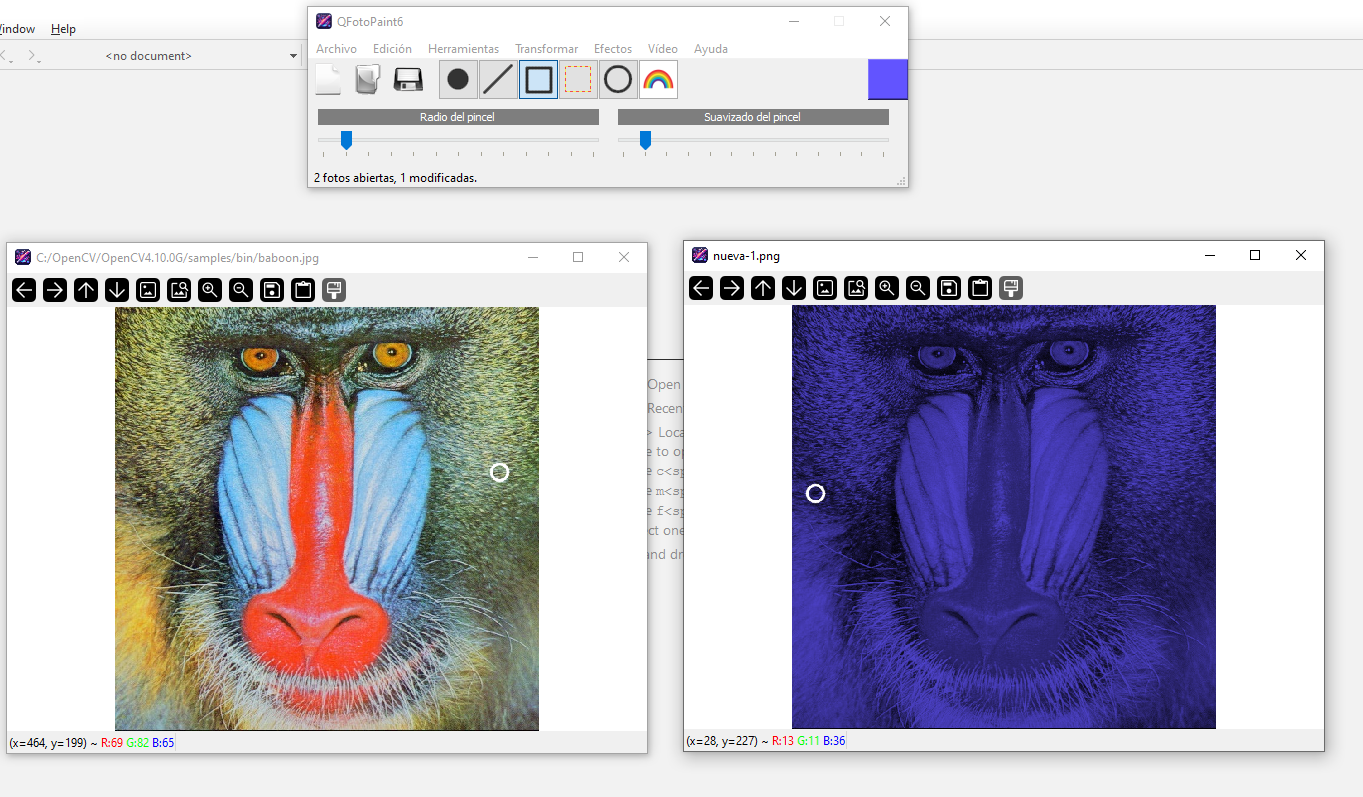
\includegraphics[width=0.8\textwidth]{imagenes/Escala-de-color.png}
\caption{Uso real de la funcionalidad X: breve descripción (ej.: menú $\to$ Herramienta $\to$ Acción).}
\label{fig:funcionalidad_nombre}
\end{figure}

Recomendaciones:
\begin{itemize}
	\item Guarda las imágenes en \texttt{Memoria/imagenes/}.
	\item Nombres descriptivos: \texttt{captura\_editar\_imagen.png}, \texttt{captura\_filtro\_blur.png}, etc.
	\item Usa \texttt{width} entre \verb|0.5\textwidth| y \verb|0.9\textwidth| según la resolución.
	\item En la leyenda indica la secuencia de acciones (ej.: ``Menú Archivo $\to$ Abrir $\to$ Seleccionar imagen'').
\end{itemize}

\subsection{Menú Archivo}

El enunciado describe el siguiente conjunto mínimo de comandos en el menú \textbf{Archivo}. A continuación se indica el estado de implementación en este proyecto.

\begin{itemize}
	\item \textbf{Nueva.} Crear una nueva imagen, especificando el tamaño y el color de fondo. \textbf{Estado:} incluida en el programa base.
	\item \textbf{Abrir.} Leer una imagen de un archivo existente, en cualquiera de los formatos admitidos por OpenCV. \textbf{Estado:} incluida en el programa base.
	\item \textbf{Guardar.} Guardar una imagen, sin necesidad de indicar el nombre. \textbf{Estado:} incluida en el programa base.
	\item \textbf{Guardar como...} Guardar una imagen, especificando el nuevo nombre. \textbf{Estado:} incluida en el programa base.
	\item \textbf{Cerrar.} Cerrar una imagen abierta. En caso de haber sido modificada, se dará la opción de guardarla. \textbf{Estado:} incluida en el programa base.
	\item \textbf{Capturar de cámara.} Capturar la imagen de una cámara de vídeo conectada al ordenador. Se puede previsualizar la entrada y capturar cuando se desee. \textbf{Estado:} implementada. \label{item:capturar_camara}
	\item \textbf{Capturar de vídeo.} Abrir una imagen que corresponda a un frame concreto dentro de un archivo de vídeo; permite previsualizar el frame y desplazarse por el vídeo. \textbf{Estado:} implementada. \label{item:capturar_video}
	\item \textbf{Nueva desde el portapapeles.} Si el portapapeles contiene una imagen, abrirla para editarla (opcional). \textbf{Estado:} implementada.
	\item \textbf{Salir.} Terminar el programa liberando memoria y dando opción a guardar imágenes modificadas. \textbf{Estado:} incluida en el programa base.
\end{itemize}

Para las funcionalidades implementadas (capturar de cámara y capturar de vídeo) se deben añadir capturas reales que ilustren su uso. A continuación se incluyen dos figuras placeholder; reemplaza los ficheros \texttt{captura\_camara.png} y \texttt{captura\_video.png} por las imágenes reales cuando las tengas.

\begin{figure}[htbp]
\centering
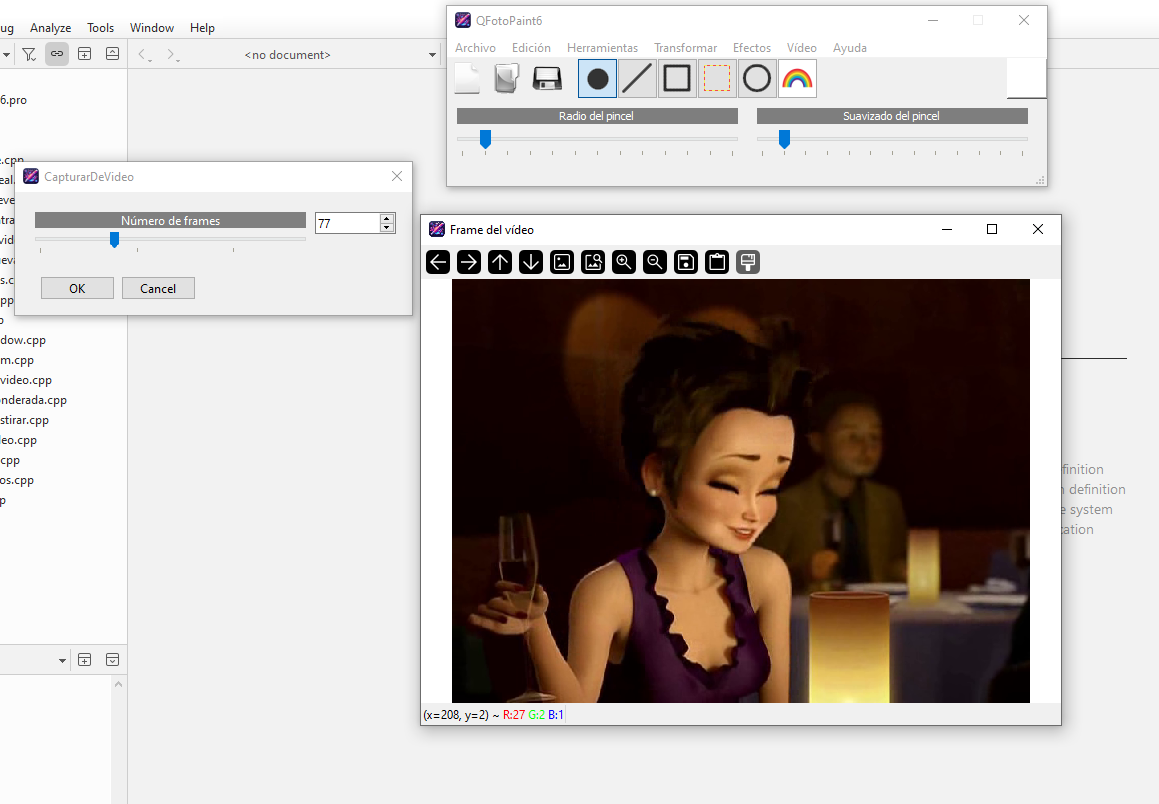
\includegraphics[width=0.75\textwidth]{imagenes/Capturar-de-video.png}
\caption{Previsualización y captura desde cámara (Menú Archivo $\to$ Capturar de cámara).}
\label{fig:captura_camara}
\end{figure}

\begin{figure}[htbp]
\centering
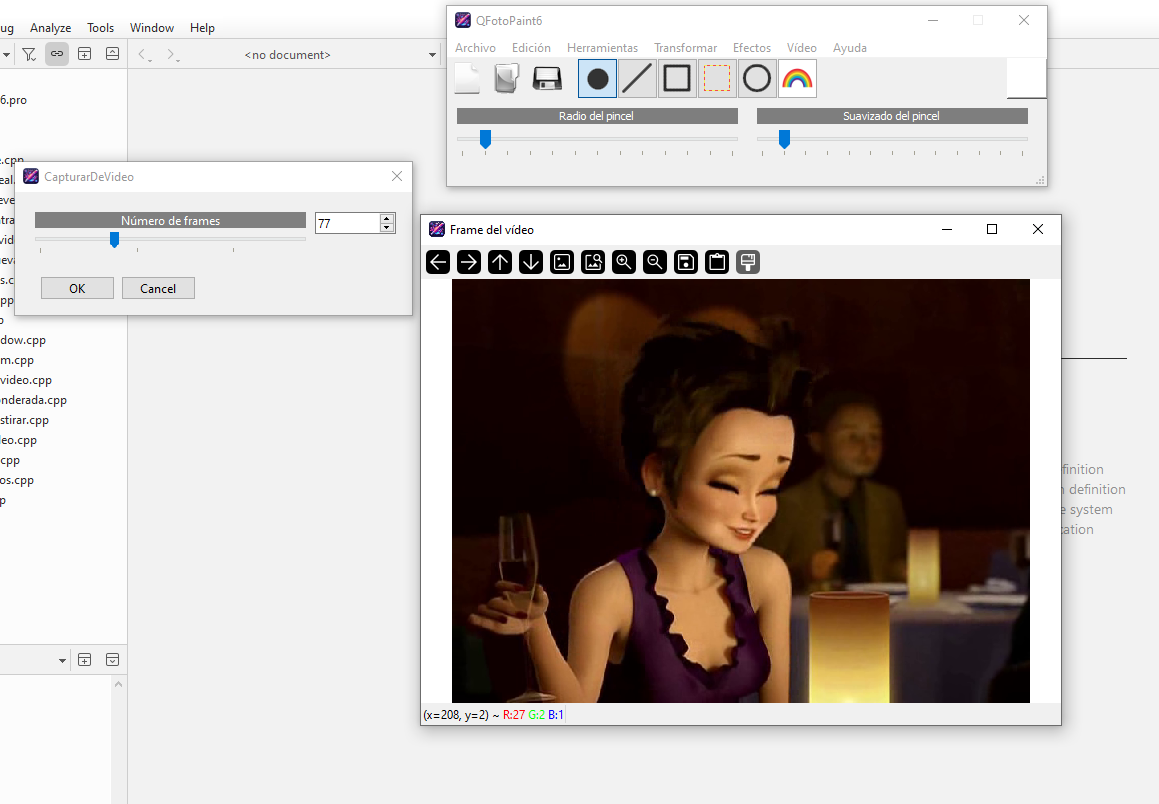
\includegraphics[width=0.75\textwidth]{imagenes/Capturar-de-video.png}
\caption{Selección de frame desde un archivo de vídeo (Menú Archivo $\to$ Capturar de vídeo).}
\label{fig:captura_video}
\end{figure}

\subsection{Menú Edición}

Las operaciones del menú \textbf{Edición} se aplican sobre la ventana activa. El enunciado pide las siguientes operaciones; a continuación se indica el estado de cada una en este proyecto.

\begin{itemize}
	\item \textbf{Deshacer.} Deshacer la última, o las n últimas, operaciones aplicadas sobre las imágenes abiertas (opcional). \textbf{Estado:} no implementada.
	\item \textbf{Seleccionar todo.} Seleccionar toda la imagen para operaciones con ROI. \textbf{Estado:} incluida en el programa base.
	\item \textbf{Copiar a nueva.} Crear una nueva imagen con el ROI de la imagen actual; si no hay ROI, copiar toda la imagen. \textbf{Estado:} incluida en el programa base.
	\item \textbf{Copiar al portapapeles.} Copiar el ROI al portapapeles del sistema (opcional). \textbf{Estado:} implementada.
	\item \textbf{Ver histograma.} Mostrar histograma (gris o por canales) con escalas en fondo. \textbf{Estado:} incluida en el programa base.
	\item \textbf{Ver histograma 2D.} Mostrar histogramas 2D agrupando canales de a 2 (opcional). \textbf{Estado:} no implementada.
	\item \textbf{Ver información.} Mostrar información relevante de la imagen (tamaño, profundidad, canales, memoria, color medio, etc.) (opcional). \textbf{Estado:} implementada.
	\item \textbf{Opciones.} Configurar opciones del programa (color actual, preguntar si guardar, etc.). \textbf{Estado:} incluida en el programa base.
\end{itemize}

De las herramientas de dibujo y selección, en este proyecto se han implementado las siguientes: rectángulo, elipse, arco iris y la herramienta de selección. A continuación hay placeholders para capturas de cada una; reemplaza los ficheros en \texttt{Memoria/imagenes/} por las capturas reales cuando las tengas.

\subsubsection{Implementación: portapapeles y ver información}

En esta subsección se describen las decisiones de implementación y las funciones clave que permiten:

\begin{itemize}
	\item \textbf{Copiar al portapapeles:} La acción "Copiar al portapapeles" está implementada en la función \texttt{copiar\_roi\_al\_portapapeles} (archivo \texttt{QFotoPaint6/imagenes.cpp}). El procedimiento es el siguiente:
	\begin{itemize}
		\item Se valida que exista una ventana activa y que la ROI no esté vacía.
		\item Se extrae la ROI como un \texttt{cv::Mat} y se convierte al formato apropiado para \texttt{QImage}:
		\begin{itemize}
			\item Imágenes BGR (3 canales): se convierten a RGB con \texttt{cv::cvtColor(..., COLOR\_BGR2RGB)} y se crea un \texttt{QImage} con \texttt{QImage::Format\_RGB888}.
			\item Imágenes BGRA (4 canales): se convierten a RGBA con \texttt{COLOR\_BGRA2RGBA} y se usa \texttt{QImage::Format\_RGBA8888}.
			\item Imágenes en escala de grises: se usa \texttt{QImage::Format\_Grayscale8}.
		\end{itemize}
		\item Se copia el \texttt{QImage} para garantizar la propiedad de los datos y se coloca en el portapapeles con \texttt{QApplication::clipboard()-\>setImage(...)}, de forma que pueda pegarse en aplicaciones del sistema (p. ej. Paint, Word) en Windows.
	\end{itemize}

	\item \textbf{Nueva desde el portapapeles:} Implementada en el slot \texttt{MainWindow::on\_actionNueva\_desde\_portapapeles\_triggered()} (archivo \texttt{QFotoPaint6/mainwindow.cpp}). Flujo principal:
	\begin{itemize}
		\item Se obtiene el portapapeles con \texttt{QApplication::clipboard()} y se comprueba que contiene una imagen con \texttt{mimeData()->hasImage()}.
		\item Se recibe la imagen como \texttt{QImage}, se convierte a \texttt{QImage::Format\_RGBA8888} y se crea un \texttt{cv::Mat} que referencia los datos.
		\item Se convierte el orden de canales a BGR con \texttt{cv::cvtColor(..., COLOR\_RGBA2BGR)} y se llama a \texttt{crear\_nueva(...)} para abrir la imagen en una nueva ventana del programa.
	\end{itemize}

	\item \textbf{Ver información de la imagen:} Implementada en el slot \texttt{MainWindow::on\_actionVer\_informacion\_triggered()} (archivo \texttt{QFotoPaint6/mainwindow.cpp}). La implementación calcula y muestra en un diálogo la siguiente información:
	\begin{itemize}
		\item Tamaño (ancho x alto), número de canales y profundidad (tipo de dato OpenCV, p. ej. \texttt{CV\_8U}, \texttt{CV\_32F}, etc.).
		\item Memoria ocupada (bytes) calculada como \texttt{m.total() * m.elemSize()}. 
		\item Color medio por canal (se usa \texttt{cv::mean(m)}). Como OpenCV almacena en BGR, se reordena a RGB para mostrarlo al usuario.
		\item Un pequeño recuadro de color generado mediante HTML en el texto enriquecido del \texttt{QMessageBox} para mostrar visualmente el color medio.
	\end{itemize}
\end{itemize}

Estas implementaciones usan la interoperabilidad entre OpenCV y Qt (conversión entre \texttt{cv::Mat} y \texttt{QImage}) y las utilidades de Qt para interactuar con el sistema (\texttt{QClipboard} y \texttt{QMessageBox}).

Si deseas, puedo añadir fragmentos de código concretos en la memoria (por ejemplo, la función completa \texttt{copiar\_roi\_al\_portapapeles}) o capturas que muestren cada opción de menú en ejecución.

\begin{figure}[htbp]
\centering
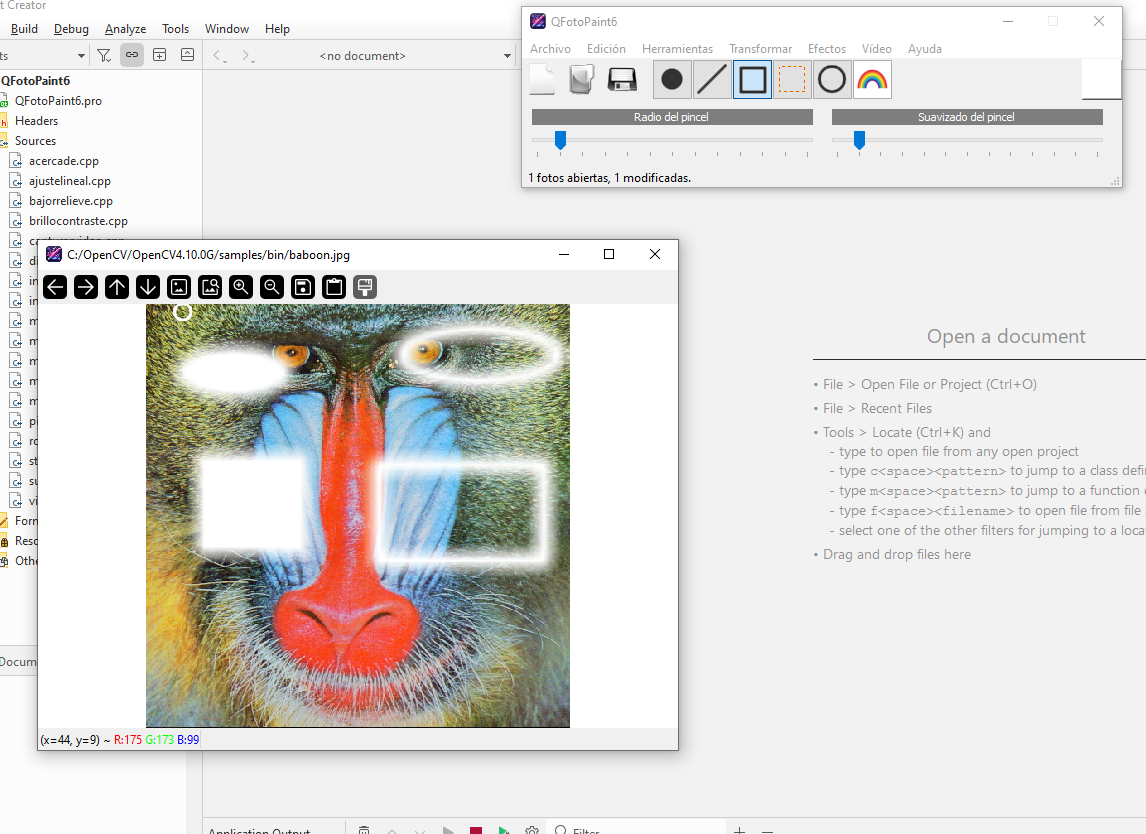
\includegraphics[width=0.7\textwidth]{imagenes/Rectangulo.png}
\caption{Dibujo de rectángulo sobre la imagen (Menú Edición $\to$ Herramientas de selección/dibujo).}
\label{fig:captura_rectangulo}
\end{figure}

\begin{figure}[htbp]
\centering
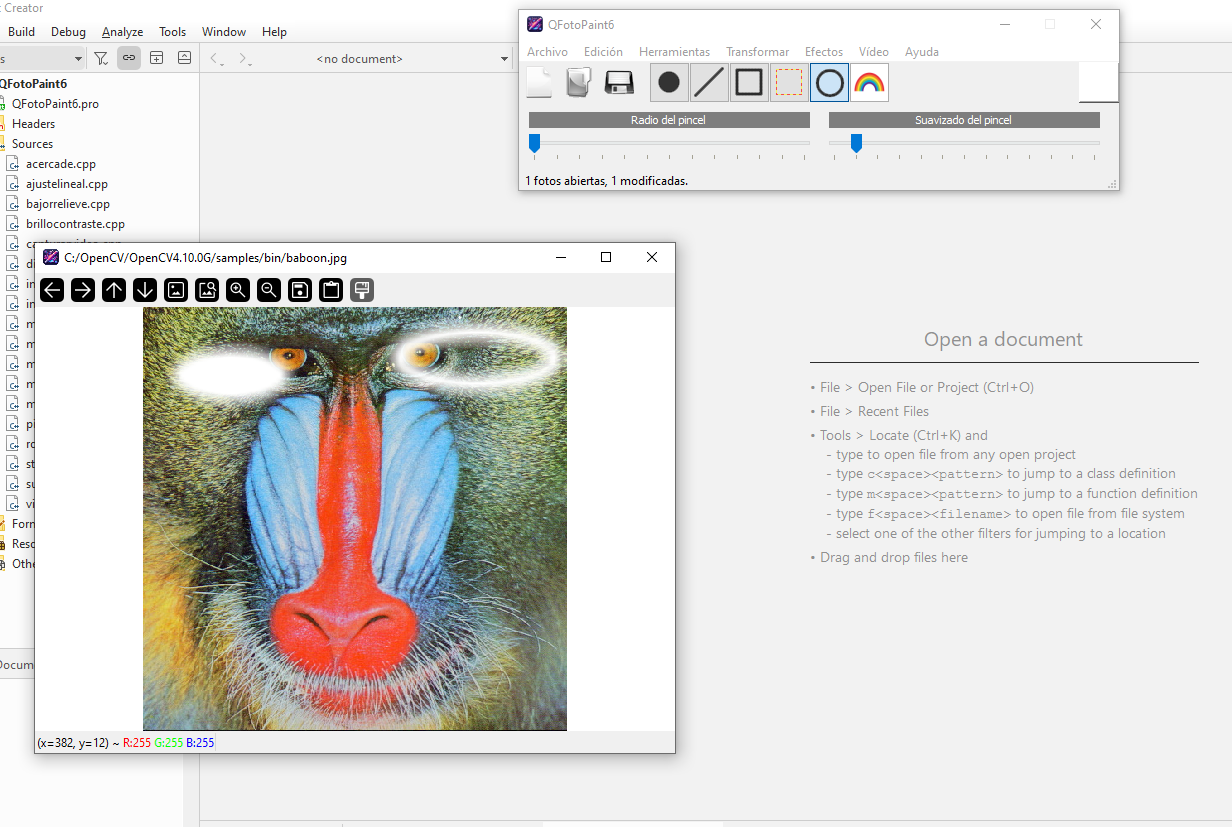
\includegraphics[width=0.7\textwidth]{imagenes/Elipse.png}
\caption{Dibujo de elipse sobre la imagen (Menú Edición $\to$ Herramientas de dibujo).}
\label{fig:captura_elipse}
\end{figure}

\begin{figure}[htbp]
\centering
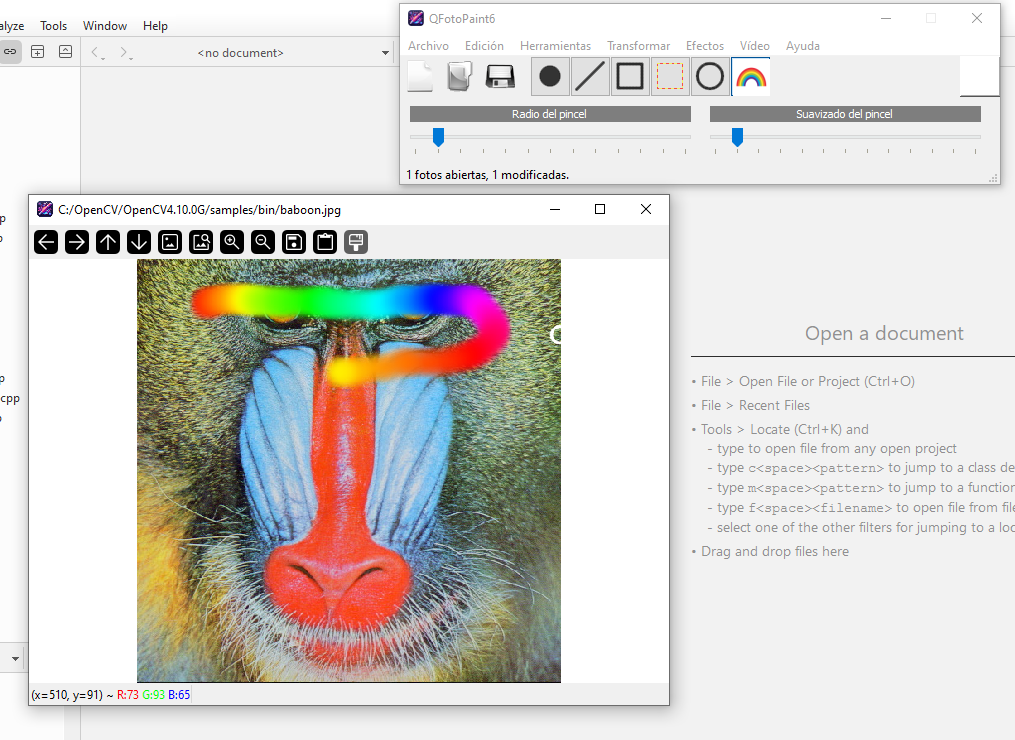
\includegraphics[width=0.7\textwidth]{imagenes/Arco-iris.png}
\caption{Aplicación del filtro "arco iris" a una región seleccionada.}
\label{fig:captura_arcoiris}
\end{figure}

\begin{figure}[htbp]
\centering
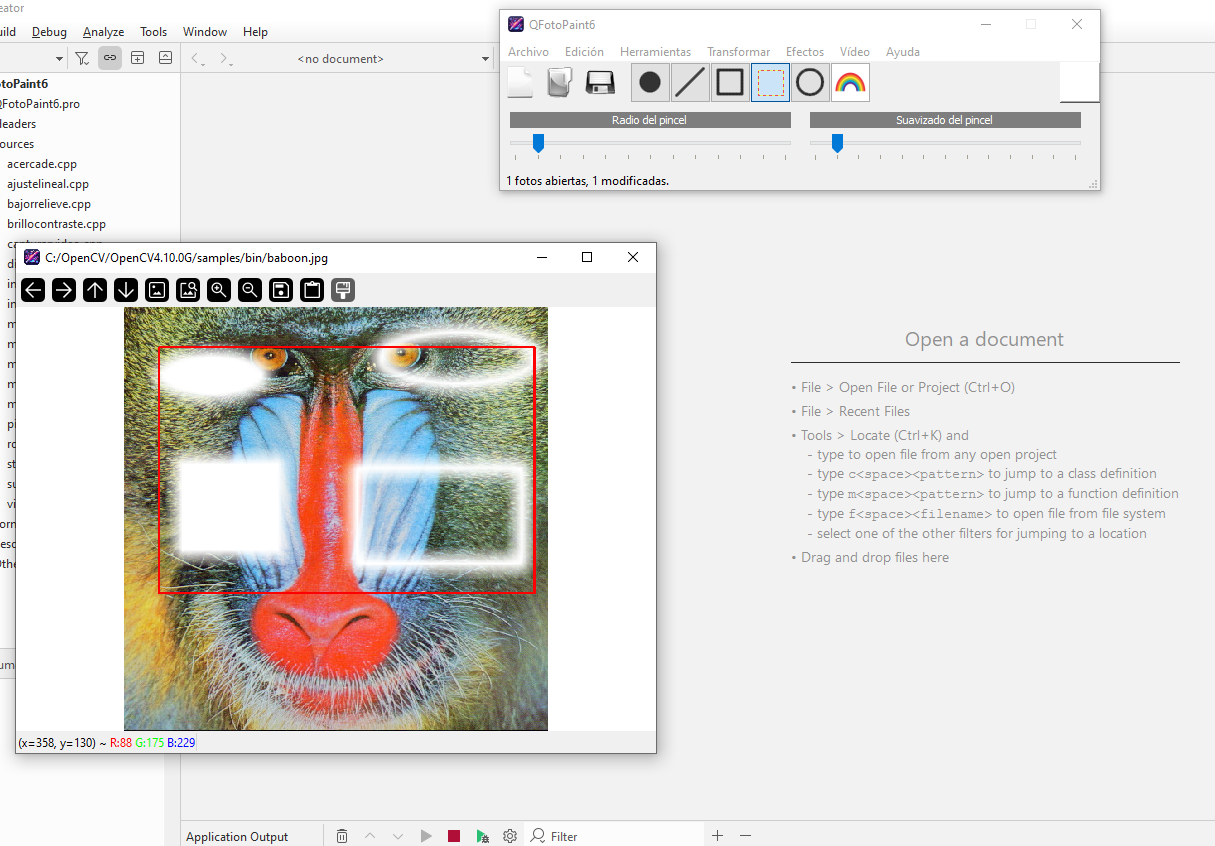
\includegraphics[width=0.7\textwidth]{imagenes/Seleccionar.png}
\caption{Uso de la herramienta de selección (seleccionar y operar sobre la ROI).}
\label{fig:captura_seleccionar}
\end{figure}

\subsection{Menú Transformar}

El menú \textbf{Transformar} contiene operaciones para modificar la apariencia y geometría de las imágenes. El enunciado solicita las siguientes operaciones; a continuación se indica el estado de implementación en este proyecto.

\begin{itemize}
	\item \textbf{Ajustar brillo/contraste/gama.} Modificar una imagen indicando brillo (suma), contraste (multiplicador) y gama. \textbf{Estado:} implementada.
	\item \textbf{Ajustar rojo/verde/azul.} Modificar cada canal por separado mediante suma/multiplicación (opcional). \textbf{Estado:} no implementada.
	\item \textbf{Ajustar matiz/saturación/luminosidad.} Ajuste de color usando internamente HLS/HSV, modificando matiz, saturación y luminosidad. \textbf{Estado:} implementada.
	\item \textbf{Ecualización del histograma.} Ecualizar histograma de forma conjunta o por canales (opcional). \textbf{Estado:} no implementada.
	\item \textbf{Ajuste lineal del histograma.} Estiramiento lineal del histograma, indicando el porcentaje de píxeles a recortar a izquierda/derecha. \textbf{Estado:} implementada.
	\item \textbf{Ecualización local.} Ecualización local del histograma con radio configurable (opcional). \textbf{Estado:} no implementada.
	\item \textbf{Rotar imagen y reescalar.} Rotar en un ángulo arbitrario y reescalar al tamaño indicado. \textbf{Estado:} no implementada.
	\item \textbf{Perspectiva.} Transformación perspectiva mediante correspondencia de 4 puntos origen-destino. \textbf{Estado:} no implementada.
	\item \textbf{Transformación de malla.} Transformaciones de malla con edición gráfica de puntos y previsualización (opcional). \textbf{Estado:} no implementada.
	\item \textbf{Convertir a escala de color.} Convertir a escala de grises o aplicar el color seleccionado. \textbf{Estado:} implementada.
	\item \textbf{Convertir a color falso.} Conversión de escala de grises a paleta de color falso (opcional). \textbf{Estado:} no implementada.
	\item \textbf{Media ponderada de dos imágenes.} Calcular la media ponderada (alfa) de dos imágenes, escalando si es necesario. \textbf{Estado:} implementada.
	\item \textbf{Curva tonal.} Transformación por curva tonal introducida gráficamente (opcional). \textbf{Estado:} no implementada.
	\item \textbf{Modelos de color.} Transformaciones entre modelos (RGB, HLS, HSV, XYZ, YUV, etc.) devolviendo imágenes por canal (opcional). \textbf{Estado:} no implementada.
	\item \textbf{Espectro.} Obtener el espectro de intensidad (magnitud de la DFT centrada) de una imagen (opcional). \textbf{Estado:} no implementada.
\end{itemize}

De las operaciones implementadas se han añadido placeholders para las capturas; reemplaza los ficheros en \texttt{Memoria/imagenes/} por las capturas reales cuando las tengas.

\begin{figure}[htbp]
\centering
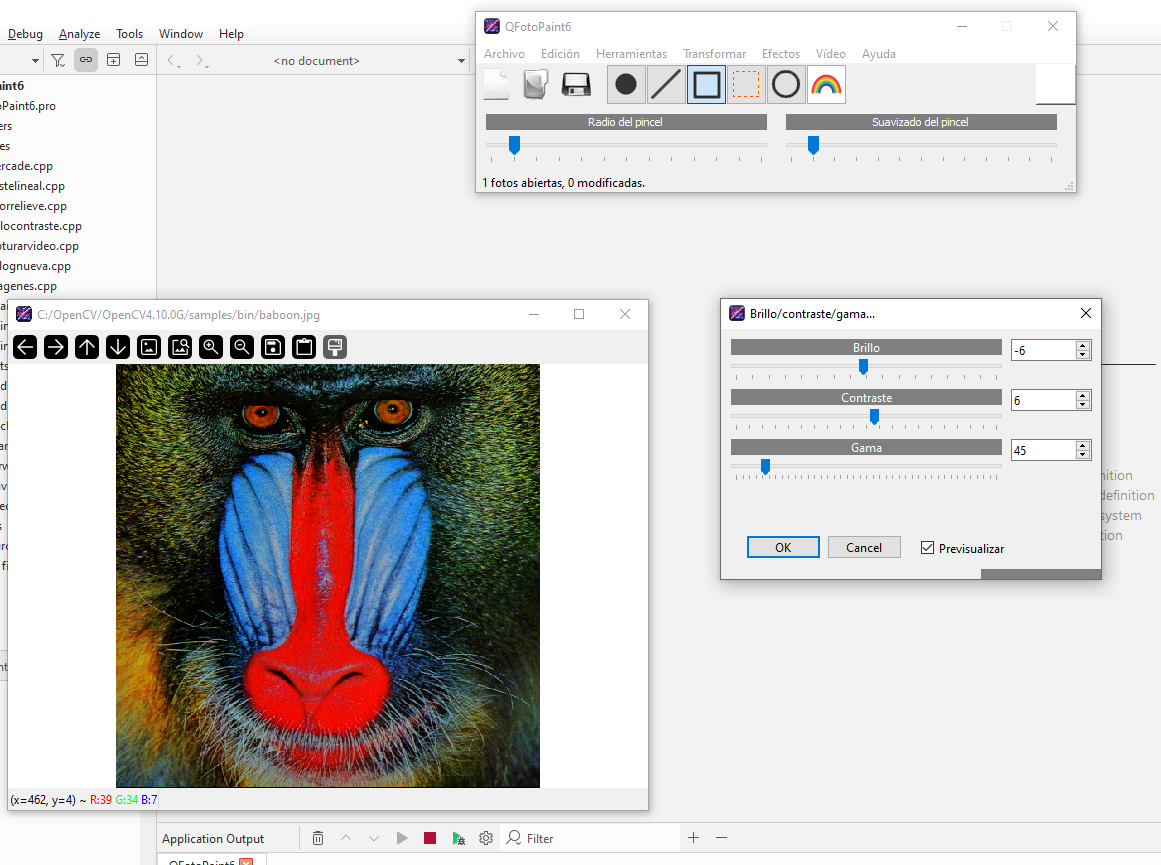
\includegraphics[width=0.75\textwidth]{imagenes/Brillo-Contraste-Gama.png}
\caption{Ajuste de brillo/contraste/gama (Menú Transformar $\to$ Ajustar brillo/contraste/gama).}
\label{fig:captura_brillo}
\end{figure}

\begin{figure}[htbp]
\centering
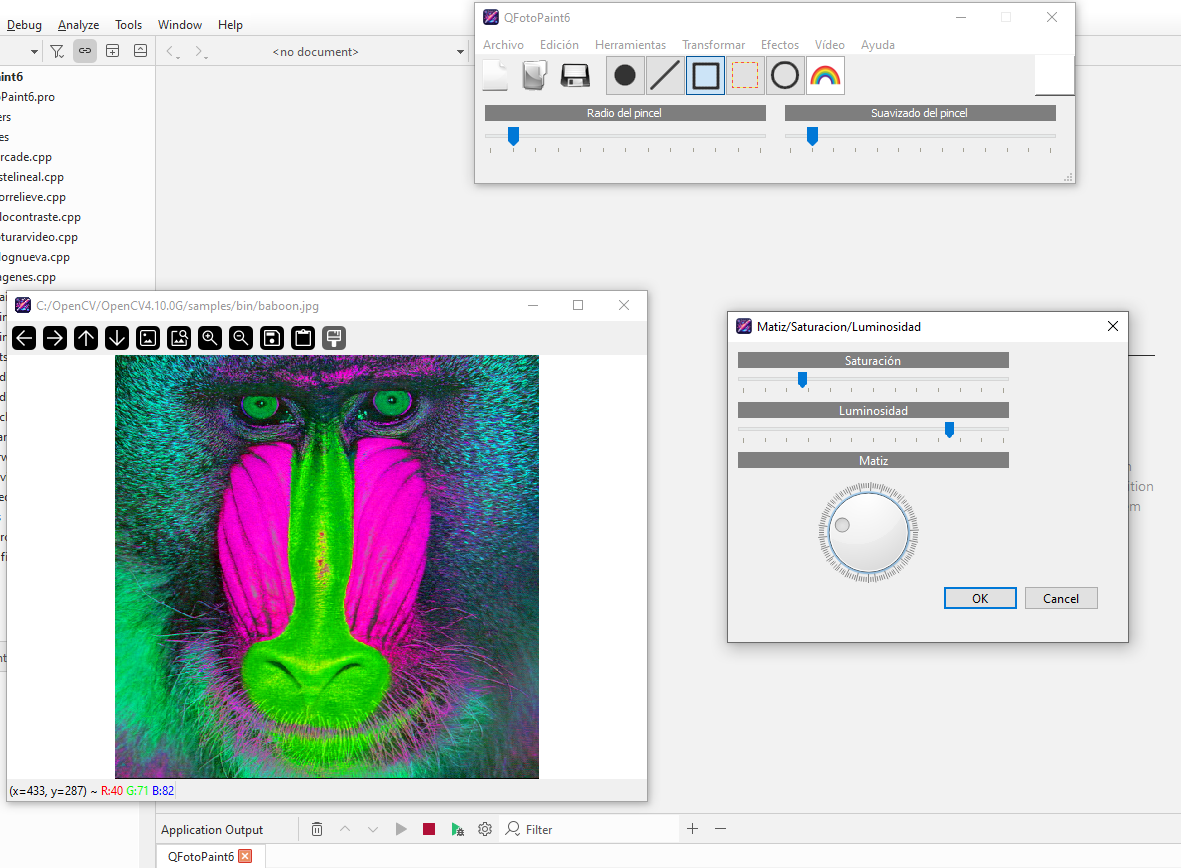
\includegraphics[width=0.75\textwidth]{imagenes/Matiz-Saturacion-Luminosidad.png}
\caption{Ajuste de matiz/saturación/luminosidad (Menú Transformar $\to$ Ajustar matiz/saturación/luminosidad).}
\label{fig:captura_hls}
\end{figure}

\begin{figure}[htbp]
\centering
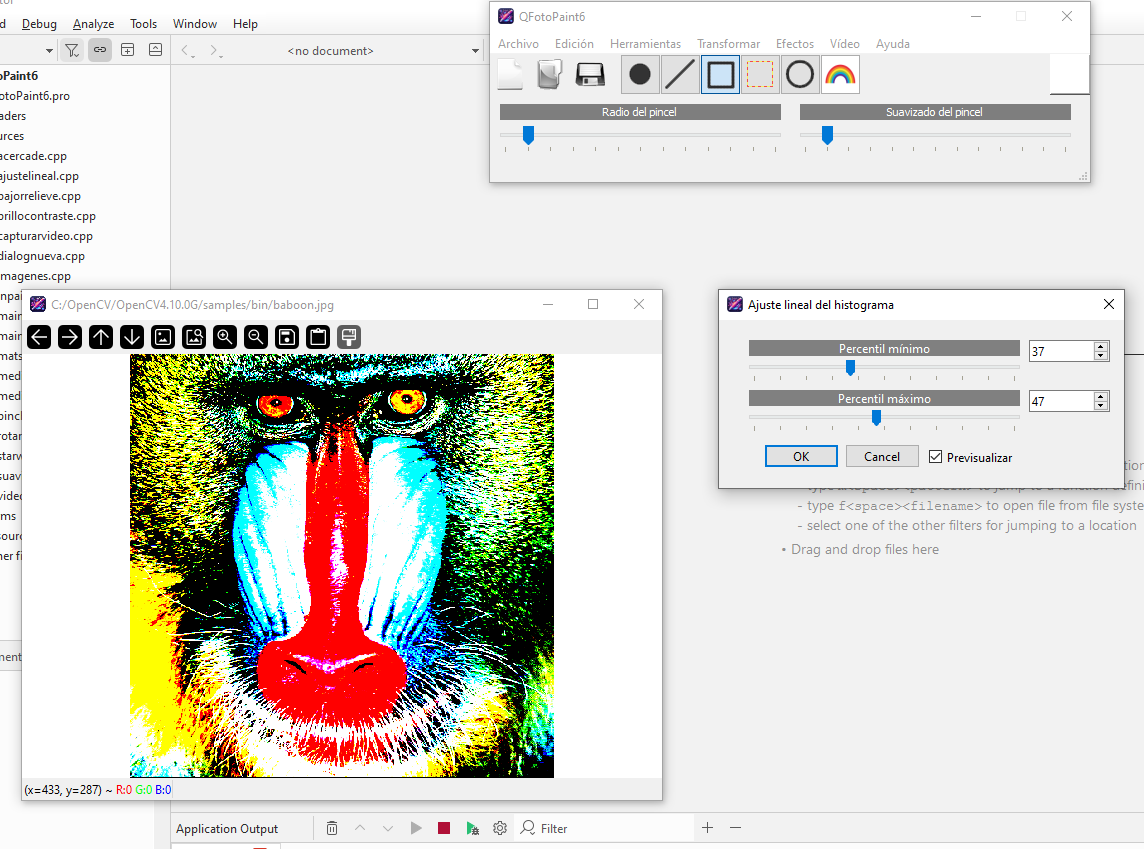
\includegraphics[width=0.75\textwidth]{imagenes/Ajuste-lineal-del-histograma.png}
\caption{Ajuste lineal del histograma (Menú Transformar $\to$ Ajuste lineal del histograma).}
\label{fig:captura_ajuste_lineal}
\end{figure}

\begin{figure}[htbp]
\centering
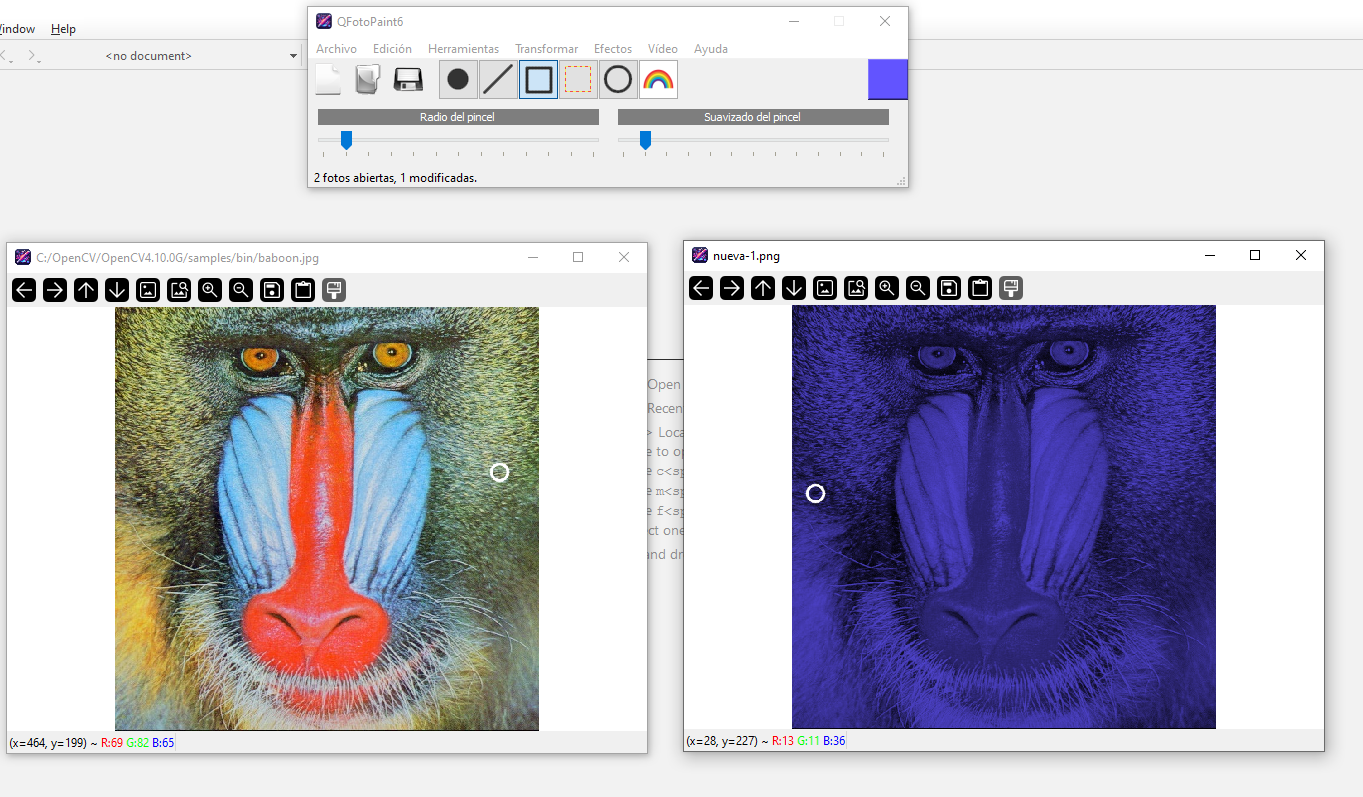
\includegraphics[width=0.75\textwidth]{imagenes/Escala-de-color.png}
\caption{Conversión a escala de color / escala de grises (Menú Transformar $\to$ Convertir a escala de color).}
\label{fig:captura_escala_color}
\end{figure}

\begin{figure}[htbp]
\centering
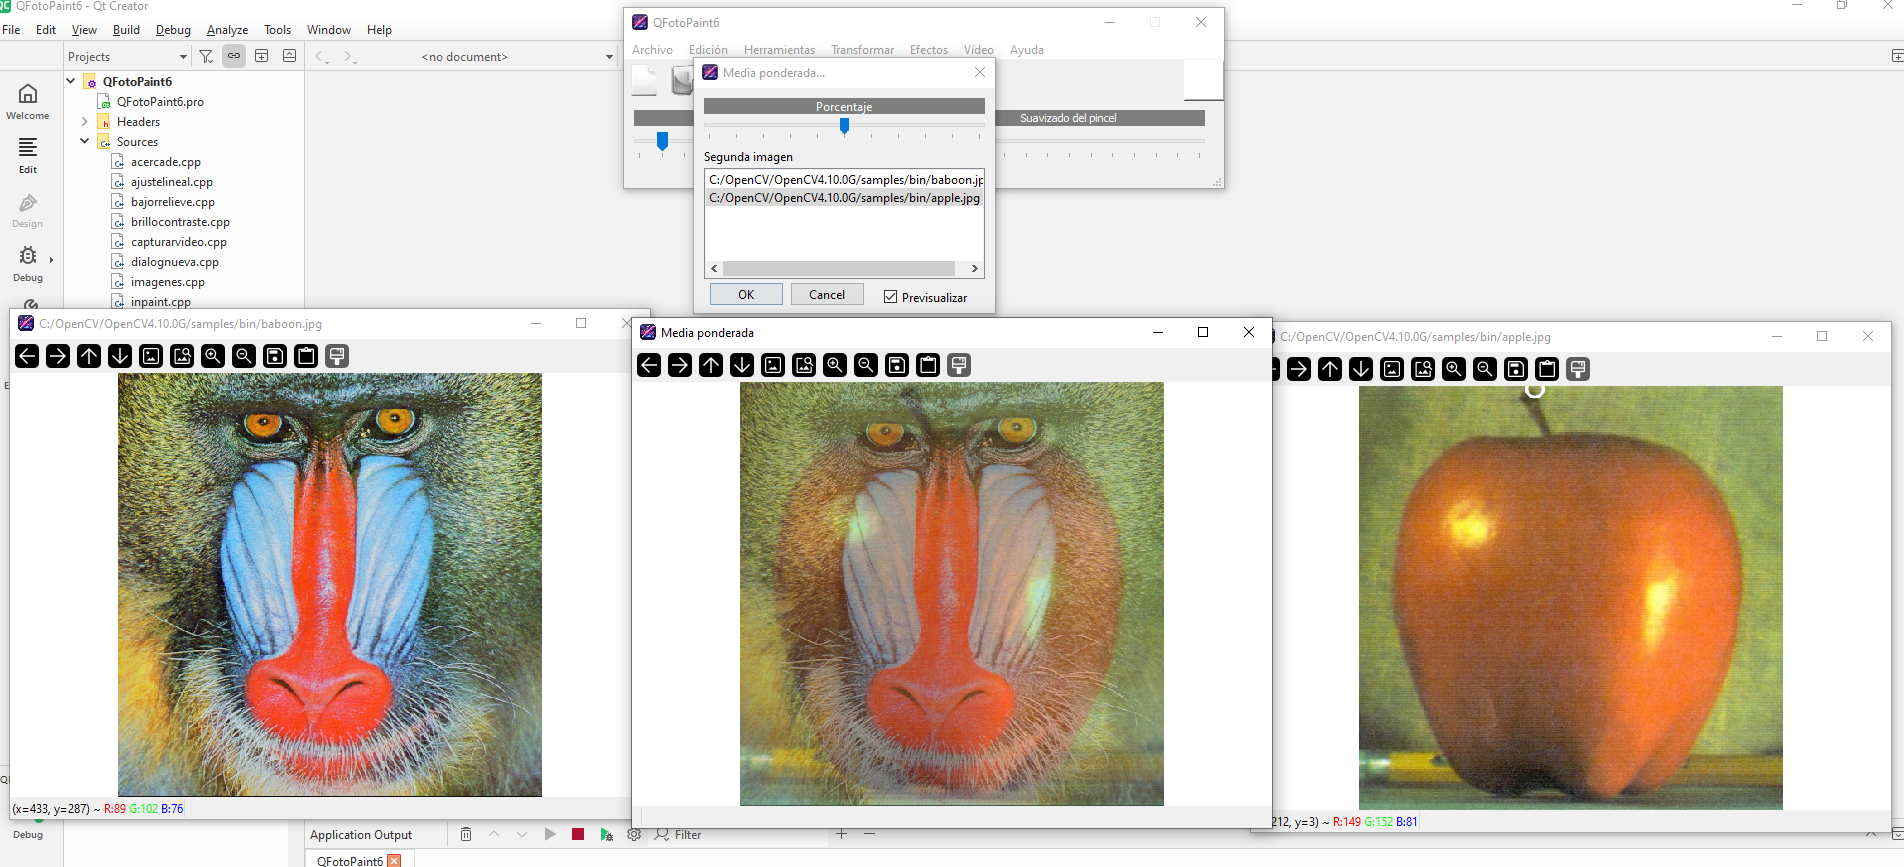
\includegraphics[width=0.75\textwidth]{imagenes/Media-Ponderada-Dos-Imaganes.png}
\caption{Media ponderada de dos imágenes (Menú Transformar $\to$ Media ponderada de dos imágenes).}
\label{fig:captura_media_ponderada}
\end{figure}

\subsection{Menú Efectos}

El menú \textbf{Efectos} incluye operaciones de filtrado y efectos visuales. El enunciado pide las siguientes operaciones; a continuación se indica el estado en este proyecto.

\begin{itemize}
	\item \textbf{Suavizado:} gaussiano, media o mediana. Aplicar el suavizado según tipo y tamaño. \textbf{Estado:} suavizado gaussiano, media y mediana implementados.
	\item \textbf{Perfilado.} Perfilar la imagen, especificando radio y porcentaje de perfilado (opcional). \textbf{Estado:} no implementado.
	\item \textbf{Bajorrelieve.} Aplicar efecto de bajorrelieve con dirección y cantidad; permitir textura o fondo gris. \textbf{Estado:} implementado.
	\item \textbf{Texto.} Añadir texto con tamaño, color y posición, con sombra difusa semitransparente (opcional). \textbf{Estado:} no implementado.
	\item \textbf{Morfología matemática.} Dilatación, erosión, abrir y cerrar con número de iteraciones (opcional). \textbf{Estado:} no implementado.
	\item \textbf{Buscar patrón.} Encontrar ocurrencias de un patrón en una imagen grande (opcional). \textbf{Estado:} no implementado.
	\item \textbf{Pinchar/estirar.} Transformaciones geométricas de pinchar/estirar indicando centro, radio y cantidad. \textbf{Estado:} implementado.
	\item \textbf{Balance de blancos.} Ajuste automático del balance de blancos (opcional). \textbf{Estado:} no implementado.
	\item \textbf{Inpaint.} Aplicar inpaint sobre zonas pintadas para borrar elementos. \textbf{Estado:} implementado.
	\item \textbf{Convolución.} Convolución arbitraria (5x5) introducida por el usuario (opcional). \textbf{Estado:} no implementado.
	\item \textbf{Geométricos.} Transformaciones geométricas tipo cilíndrica, acristalado, etc. (opcional). \textbf{Estado:} no implementado.
\end{itemize}

A continuación hay placeholders para las capturas de las operaciones implementadas; reemplaza los ficheros en \texttt{Memoria/imagenes/} por las capturas reales cuando las tengas.

\begin{figure}[htbp]
\centering
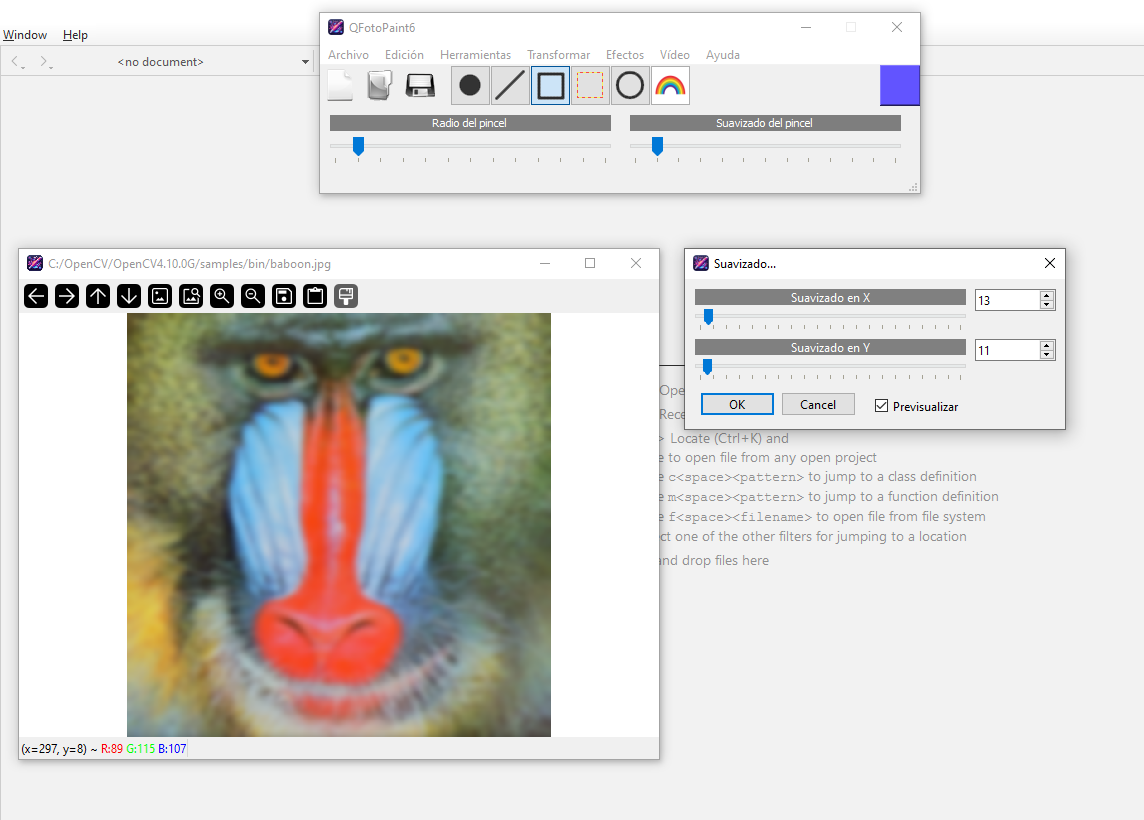
\includegraphics[width=0.7\textwidth]{imagenes/Suavizado-gausiano.png}
\caption{Suavizado gaussiano aplicado a una imagen (Menú Efectos $\to$ Suavizado).}
\label{fig:captura_suavizado_gaussiano}
\end{figure}

\begin{figure}[htbp]
\centering
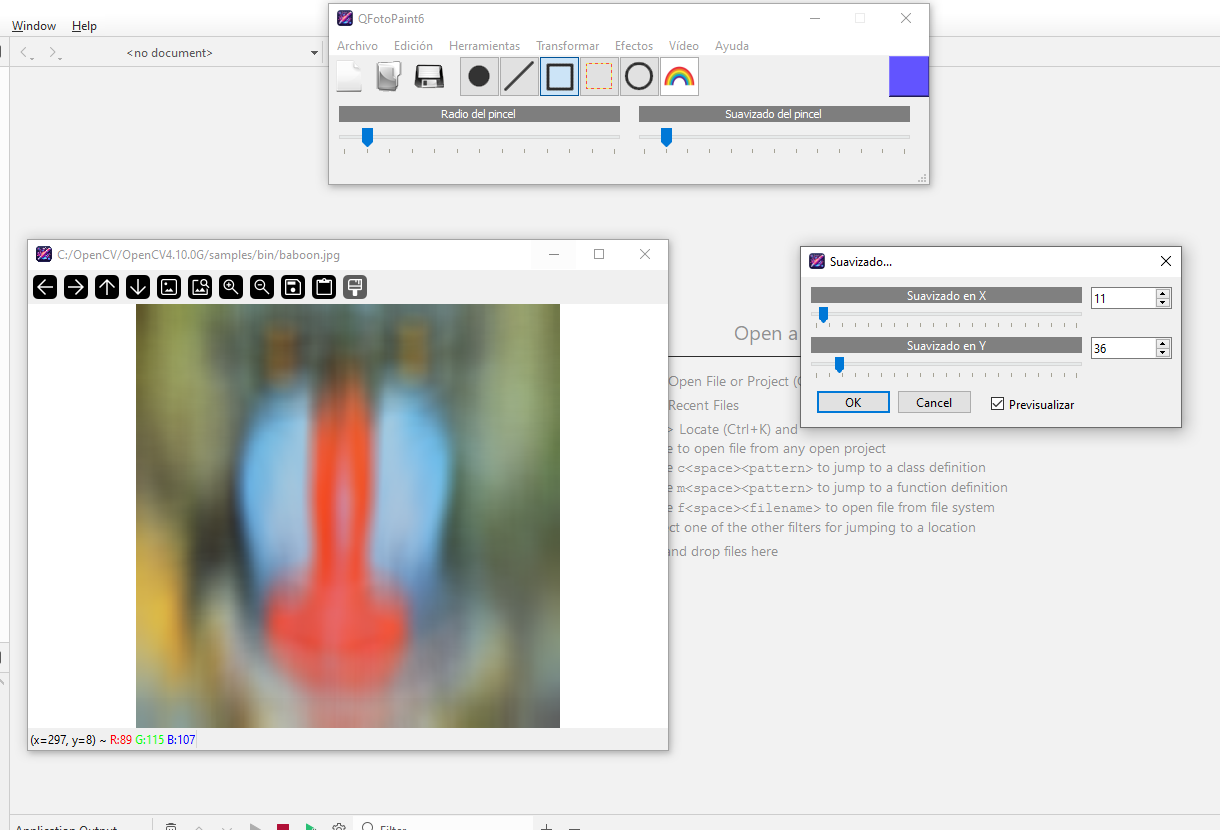
\includegraphics[width=0.7\textwidth]{imagenes/Suavizado-media.png}
\caption{Suavizado por media aplicado a una imagen (Menú Efectos $\to$ Suavizado).}
\label{fig:captura_suavizado_media}
\end{figure}

\begin{figure}[htbp]
\centering
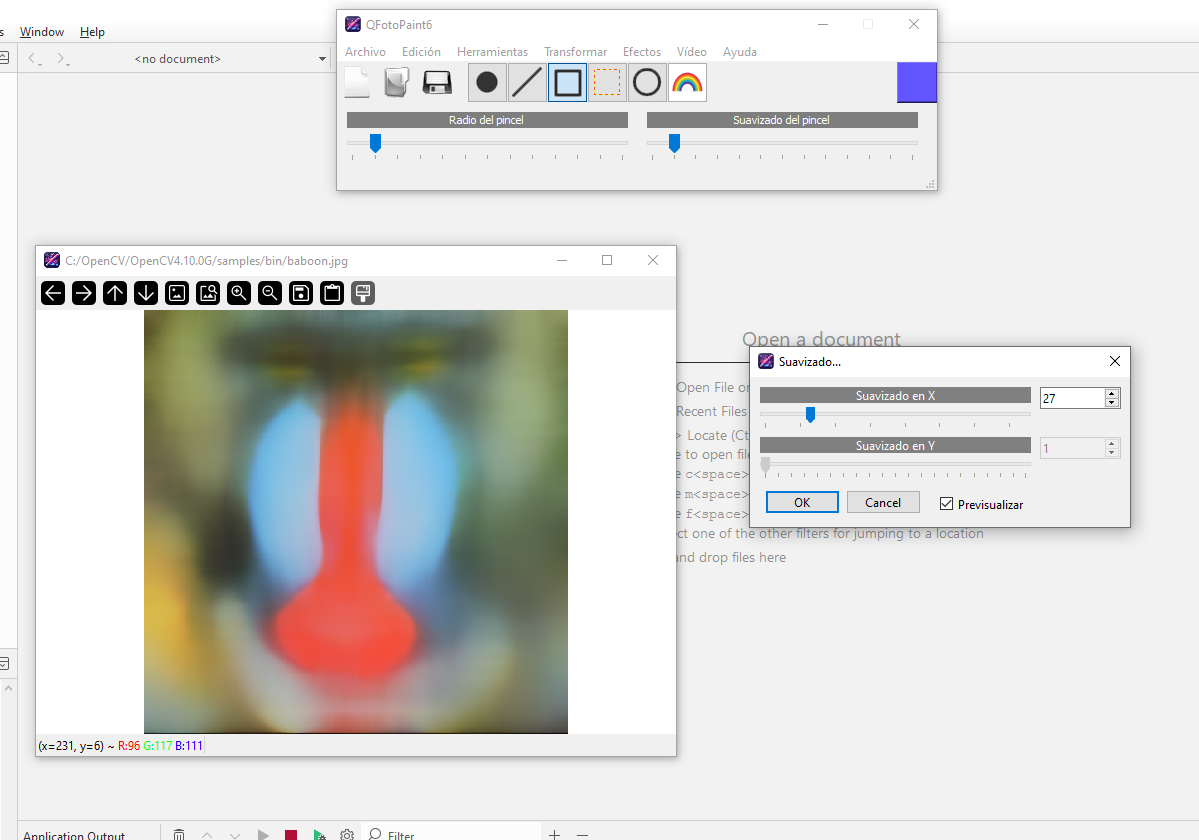
\includegraphics[width=0.7\textwidth]{imagenes/Suavizado-mediana.png}
\caption{Suavizado por mediana aplicado a una imagen (Menú Efectos $\to$ Suavizado).}
\label{fig:captura_suavizado_mediana}
\end{figure}

\begin{figure}[htbp]
\centering
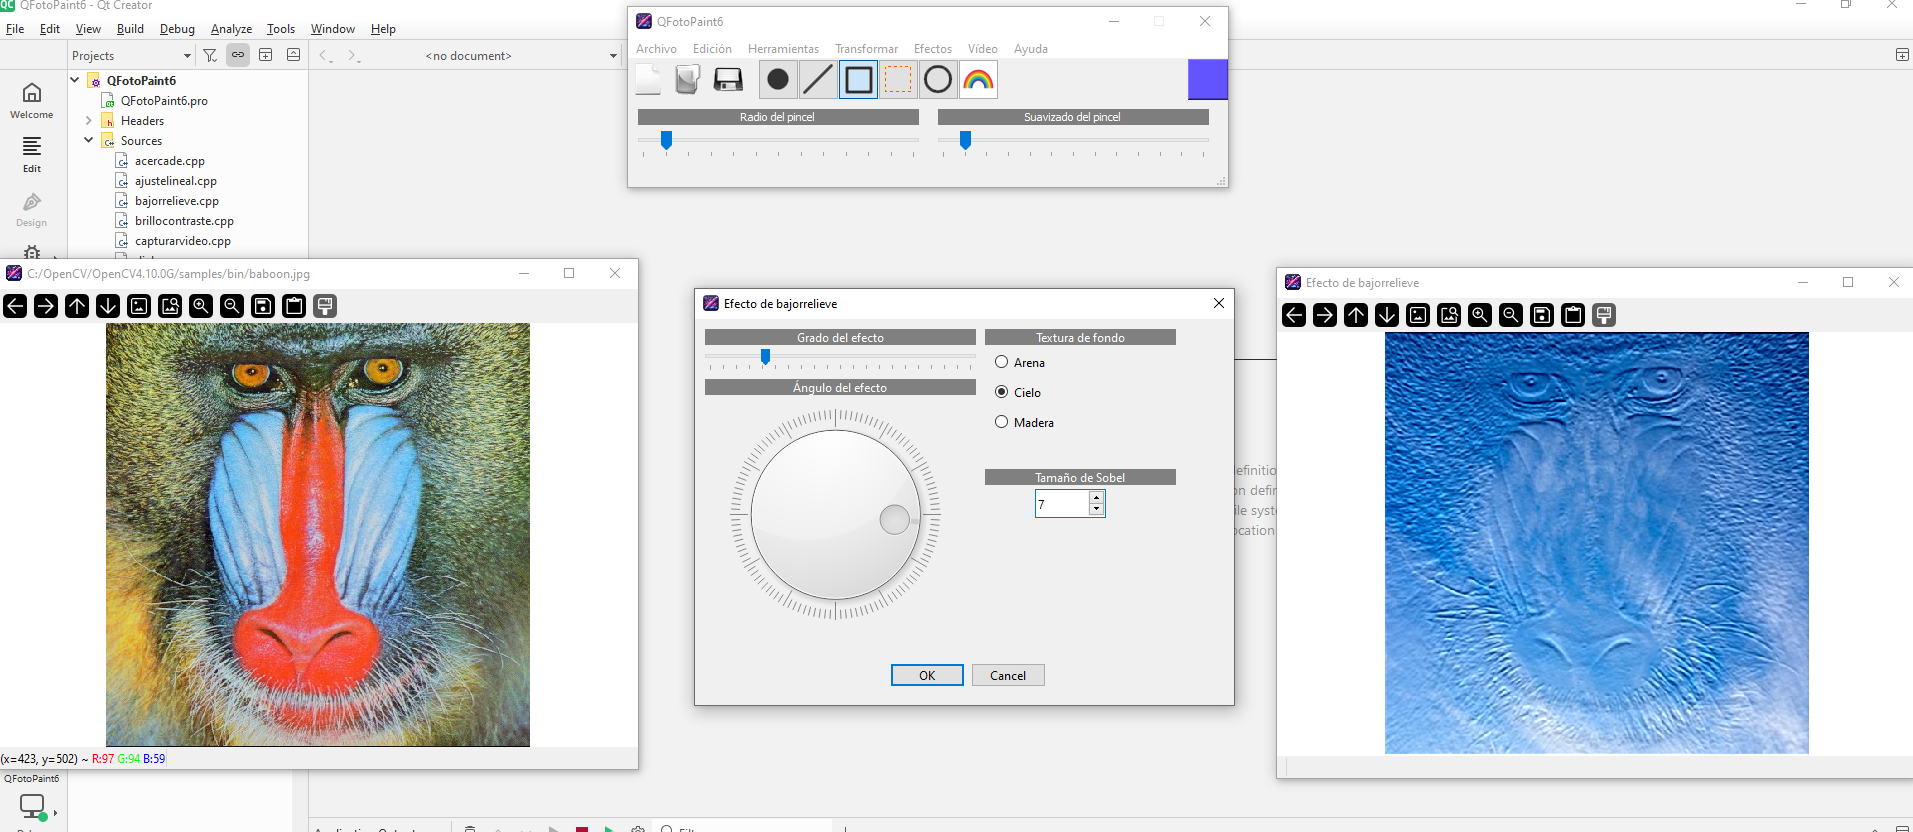
\includegraphics[width=0.7\textwidth]{imagenes/Bajorrelieve.png}
\caption{Efecto bajorrelieve aplicado (Menú Efectos $\to$ Bajorrelieve).}
\label{fig:captura_bajorrelieve}
\end{figure}

\begin{figure}[htbp]
\centering
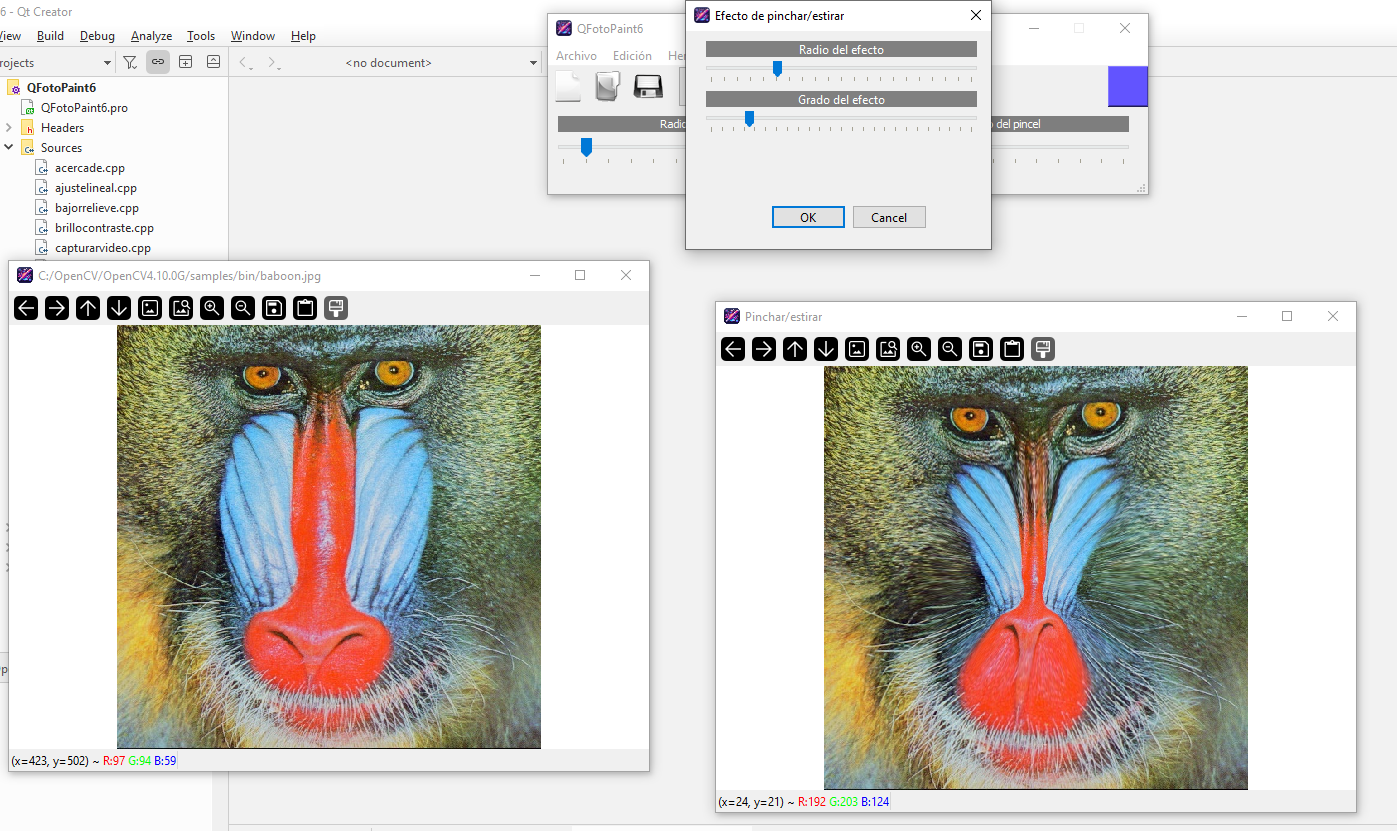
\includegraphics[width=0.7\textwidth]{imagenes/Pinchar-estirar.png}
\caption{Transformación de pinchar/estirar (Menú Efectos $\to$ Pinchar/estirar).}
\label{fig:captura_pinchar_estirar}
\end{figure}

\begin{figure}[htbp]
\centering
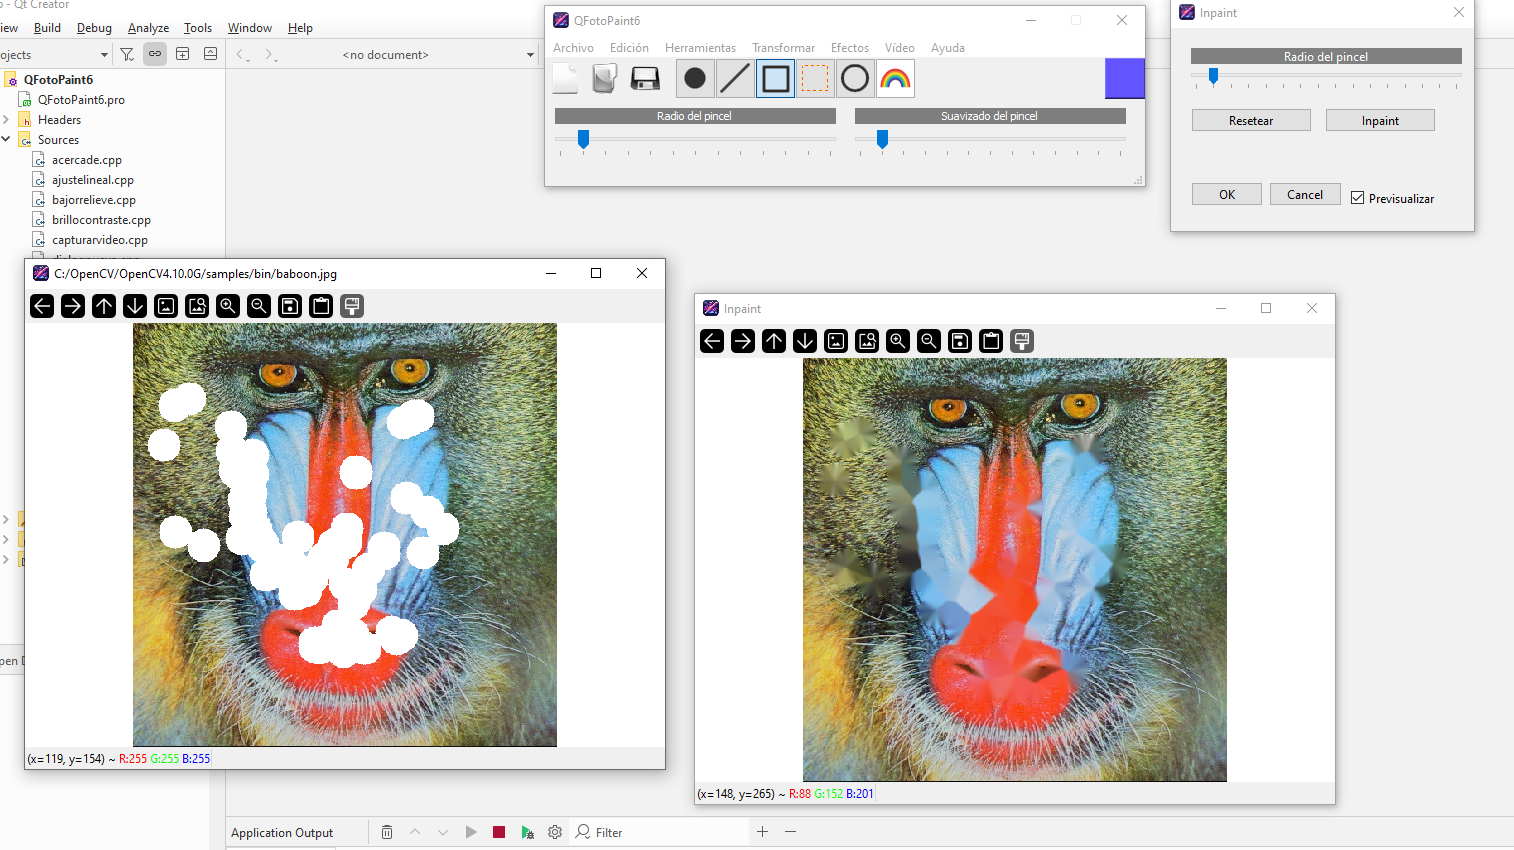
\includegraphics[width=0.7\textwidth]{imagenes/Inpaint.png}
\caption{Uso de Inpaint para borrar una región (Menú Efectos $\to$ Inpaint).}
\label{fig:captura_inpaint}
\end{figure}

\subsection{Menú Vídeo}

Las operaciones relacionadas con vídeo se agrupan en tres bloques: \textbf{Imagen a Vídeo}, \textbf{Vídeo a Imagen} y \textbf{Vídeo a Vídeo}. A continuación se resumen las operaciones pedidas en el enunciado y el estado de implementación en este proyecto.

\paragraph{Imagen a Vídeo}
\begin{itemize}
	\item \textbf{Rotar imagen.} Dada una imagen, generar un vídeo con una rotación completa de la misma. \textbf{Estado:} no implementada.
	\item \textbf{Transición entre imágenes.} Dadas dos imágenes, crear un vídeo con una transición suave (escalado, suavizado, alfa-blending, etc.) (opcional). \textbf{Estado:} no implementada.
	\item \textbf{Star Wars.} Dada una imagen y un texto de usuario, generar un vídeo donde el texto aparece de abajo hacia arriba con transformación perspectiva (títulos estilo "Star Wars"). \textbf{Estado:} implementada.
\end{itemize}

\paragraph{Vídeo a Imagen}
\begin{itemize}
	\item \textbf{Media.} Obtener la media por píxel de los frames considerados. \textbf{Estado:} no implementada.
	\item \textbf{Mínima/Máxima.} Obtener imágenes con el mínimo y el máximo por píxel (opcional). \textbf{Estado:} no implementada.
	\item \textbf{Movimiento.} Señalar zonas con más movimiento acumulado entre frames (opcional). \textbf{Estado:} no implementada.
	\item \textbf{Caras.} Generar una imagen con las caras encontradas en el vídeo (opcional). \textbf{Estado:} no implementada.
\end{itemize}

\paragraph{Vídeo a Vídeo}
\begin{itemize}
	\item \textbf{Copiar con efectos.} Copiar una secuencia aplicando una transformación o efecto (opcional). \textbf{Estado:} no implementada.
	\item \textbf{Suavizado temporal.} Cada frame es la media de los $n$ frames anteriores (opcional). \textbf{Estado:} no implementada.
	\item \textbf{Detección de caras.} Generar un vídeo donde las caras detectadas se marcan con rectángulos (opcional). \textbf{Estado:} no implementada.
\end{itemize}

De las operaciones anteriores, en este proyecto se ha implementado la opción \textbf{Star Wars}. A continuación se añade un placeholder para la captura de pantalla correspondiente; reemplaza el fichero \texttt{imagenes/Star-wars.png} por la imagen real cuando la tengas.

\begin{figure}[htbp]
\centering
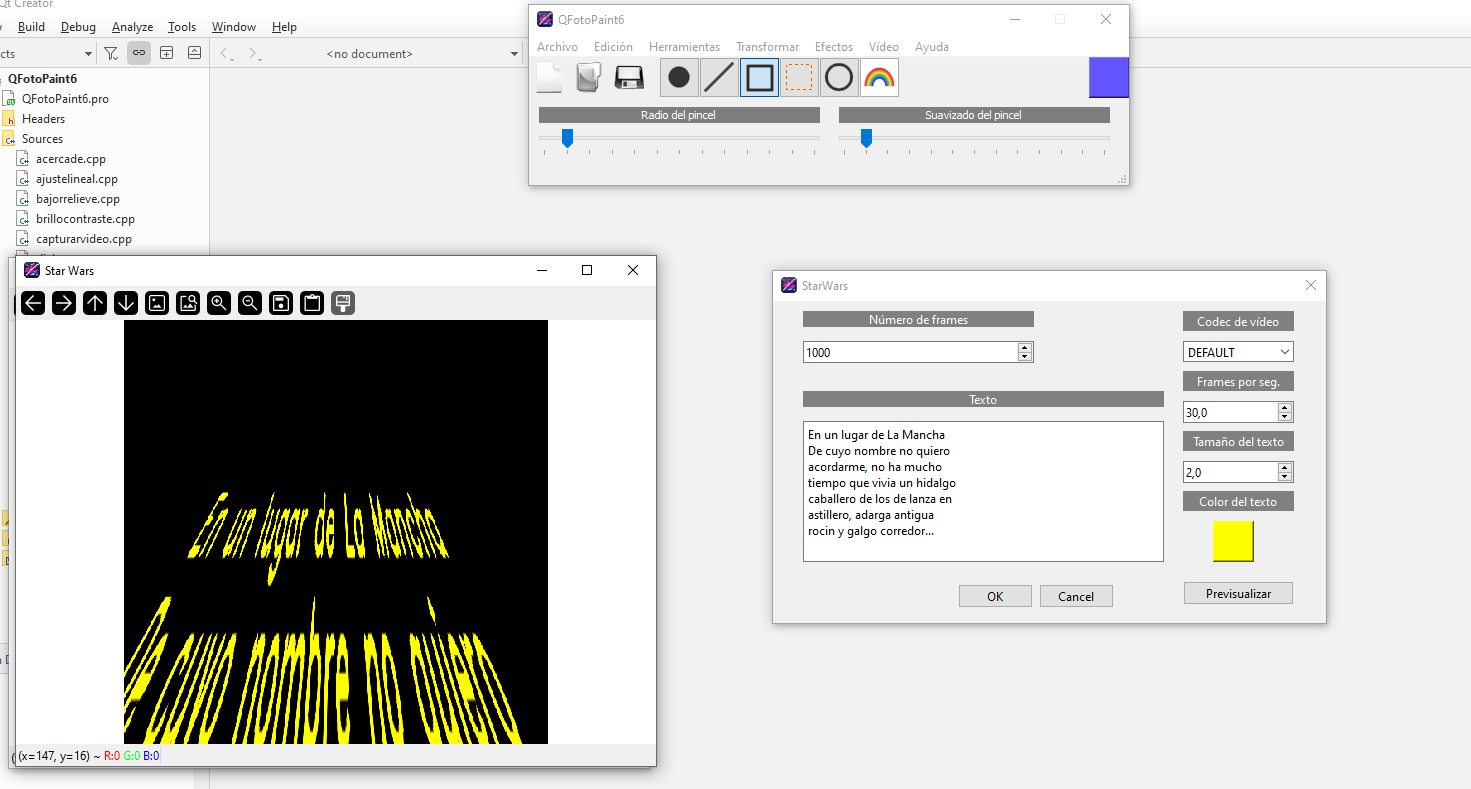
\includegraphics[width=0.8\textwidth]{imagenes/Star-wars.png}
\caption{Generación de vídeo estilo "Star Wars" (Imagen a Vídeo $\to$ Star Wars).}
\label{fig:captura_star_wars}
\end{figure}


\section{Diseño de la aplicación}

Esta sección describe el diseño general de la aplicación QFotoPaint6.

\subsection{Arquitectura}

- \textbf{Interfaz gráfica:} implementada con Qt (widgets y acciones en \texttt{mainwindow.*}).
- \textbf{Procesamiento de imagen:} funciones agrupadas en el módulo \texttt{imagenes.h/cpp}, usando OpenCV para operaciones sobre \texttt{cv::Mat}.
- \textbf{Vídeo y captura:} funcionalidades específicas en \texttt{video.h/cpp} que usan OpenCV (\texttt{VideoCapture}, \texttt{VideoWriter}).
- \textbf{Comunicación Qt / OpenCV:} conversiones entre \texttt{cv::Mat} y \texttt{QImage} para integrar con la API de Qt (por ejemplo para el portapapeles y visualización).

\subsection{Organización del código}

- Ficheros principales de UI: \texttt{mainwindow.cpp/.h} y el recurso \texttt{recursos.qrc}.
- Funcionalidades de imagen: \texttt{imagenes.h} (interfaz) y \texttt{imagenes.cpp} (implementación).
- Funcionalidades de vídeo/cámara: \texttt{video.h} y \texttt{video.cpp}.
- Ventanas de diálogo y utilidades: ficheros como \texttt{dialognueva.*}, \texttt{capturarvideo.*}, etc.

\subsection{Decisiones de diseño relevantes}

- Se mantiene un array estático \texttt{foto[MAX\_VENTANAS]} para gestionar las ventanas/imagenes abiertas, simplificando el control y la numeración de ventanas.
- Para integrar con Qt y el portapapeles se realizan conversiones controladas a \texttt{QImage} copiando los datos cuando es necesario para evitar problemas de propiedad de memoria.
- Se emplean callbacks de OpenCV (HighGUI) para manejar eventos de ratón sobre las ventanas de imagen, lo que mantiene la lógica de interacción separada de la GUI de Qt.

\section{Resolución de los problemas más relevantes}

En esta sección se describen los problemas más relevantes encontrados durante el desarrollo y cómo se han resuelto.

\subsection{Conversión entre \texttt{cv::Mat} y \texttt{QImage}}

Problema: OpenCV usa matrices en orden BGR/BGRA y Qt espera RGB/RGBA en ciertos formatos; además la memoria subyacente puede ser gestionada por OpenCV, lo que puede provocar accesos a memoria liberada si no se copian los datos.

Solución: Antes de crear un \texttt{QImage} se convierte el orden de canales (p. ej. \texttt{COLOR\_BGR2RGB} o \texttt{COLOR\_BGRA2RGBA}) y se realiza una copia con \texttt{QImage::copy()} cuando se va a transferir al portapapeles o a Qt para garantizar la propiedad de los datos.

\subsection{Gestión de múltiples ventanas}

Problema: controlar el foco y el orden de múltiples ventanas creadas con HighGUI de OpenCV.

Solución: se utiliza el array global \texttt{foto[]} con un campo \texttt{orden} que se incrementa cada vez que una ventana obtiene foco; la función \texttt{foto\_activa()} devuelve la ventana con mayor orden.

\subsection{Captura de cámara y sincronización}

Problema: capturar frames desde la cámara y permitir operaciones como acumulado de media sin bloquear la interfaz.

Solución: el módulo \texttt{video.cpp} encapsula la lógica de captura con \texttt{VideoCapture}. Las funciones devuelven controles sencillos (por ejemplo, número de ms entre frames) y se usan ventanas de OpenCV para previsualizar; las operaciones de procesado (media, rotación, exportación) se realizan en funciones separadas para evitar entrelazar la lógica de captura y la de procesamiento.

\subsection{Compatibilidad de formatos al copiar al portapapeles}

Problema: el portapapeles del sistema puede requerir diferentes formatos según la aplicación destino.

Solución: se soportan conversiones para imágenes de 1, 3 y 4 canales y se colocan en el portapapeles como \texttt{QImage}; en Windows esto permite pegar en Paint y otras aplicaciones que aceptan imágenes.

\section{Listado del código}

Se incluyen a continuación los listados completos de los módulos solicitados. Los ficheros se muestran con numeración de líneas para facilitar la revisión.

\subsection{imagenes.h}
\lstinputlisting[language=C++,caption={imagenes.h}]{..\QFotoPaint6\imagenes.h}

\subsection{imagenes.cpp}
\lstinputlisting[language=C++,caption={imagenes.cpp}]{..\QFotoPaint6\imagenes.cpp}

\subsection{video.h}
\lstinputlisting[language=C++,caption={video.h}]{..\QFotoPaint6\video.h}

\subsection{video.cpp}
\lstinputlisting[language=C++,caption={video.cpp}]{..\QFotoPaint6\video.cpp}

% Nota: las rutas son relativas al directorio \texttt{Memoria/}. Si el compilador LaTeX no encuentra los ficheros, ajuste la ruta relativa.

\section{Pruebas y ejemplos de uso}

Se muestran a continuación ejemplos de uso de las funcionalidades implementadas y pequeñas pruebas realizadas.

\subsection{Copiar al portapapeles / Nueva desde el portapapeles}

Procedimiento de prueba:
\begin{enumerate}
\item Abrir una imagen en QFotoPaint6 (Menú Archivo $\to$ Abrir).
\item Seleccionar una región con la herramienta de selección (Menú Edición $\to$ Seleccionar).
\item Ejecutar "Copiar al portapapeles" (Menú Edición $\to$ Copiar al portapapeles).
\item Abrir Paint u otra aplicación y pegar (Ctrl+V). Comprobar que la imagen aparece con el contenido de la ROI.
\item En QFotoPaint6 ejecutar "Nueva desde el portapapeles" (Menú Archivo $\to$ Nueva desde el portapapeles) para verificar que se abre una nueva ventana con la imagen del portapapeles.
\end{enumerate}

\subsection{Ver información}

Prueba rápida:
\begin{itemize}
\item Abrir una imagen y ejecutar "Ver información" (Menú Edición $\to$ Ver información...).
\item Comprobar que el cuadro resultante contiene: tamaño, profundidad, canales, tamaño en memoria, (opcional) tamaño en disco y color medio con recuadro de color.
\end{itemize}

\subsection{Ejemplo: generación de vídeo rotando una imagen}

Comprobación funcional básica:
\begin{enumerate}
\item Abrir una imagen y ejecutar la opción correspondiente en el menú Vídeo (Imagen a Vídeo $\to$ Rotar imagen).
\item Ver en pantalla la previsualización y comprobar que se crea el fichero de salida si se solicitó guardar.
\end{enumerate}

Incluye en la memoria capturas de pantalla de las pruebas realizadas para facilitar la evaluación.

\section{Conclusiones}

- Se han integrado correctamente OpenCV y Qt para proporcionar una herramienta de edición con funcionalidades de imagen y vídeo.
- Las operaciones de conversión entre formatos y la gestión del portapapeles se realizaron garantizando la propiedad de los datos para evitar errores de memoria.
- El diseño con el array global \texttt{foto[]} simplifica la gestión de ventanas en el contexto de la práctica, aunque en un producto a mayor escala podría optarse por un diseño orientado a objetos con gestión dinámica de ventanas.
- Trabajo futuro: añadir tests automatizados, un sistema de deshacer/rehacer y una interfaz Qt nativa para todas las opciones (evitar depender de HighGUI para eventos de ratón si se busca uniformidad en la UX).

Estas conclusiones resumen el trabajo realizado y los puntos de mejora identificados durante la práctica.


\end{document}